\section{Item Interactions}
\label{sec:items}
Items are interactive objects that the player can pick up and use in different situations, or drop.

\subsection{Item on Character}
In the game, the player will be able to acquire certain items which can be used on characters (including themselves). These items can effect the player and NPCs in many ways: they may effect their abilities during yelling contests, effect how they move through the 3D game world, or effect how the player views the world. In the case of items being used on NPCs, these interactions may be tied to scenarios or have the possibility of affecting the \textbf{friendship} the player has with the character positively or negatively.

\subsubsection{Effects For Yelling Contest}
As described in the Yelling Contest section, the player's \textbf{D.I.S.S.} attributes have an effect on different aspects of the game. The player can use items to buff/debuff these attributes to give them an advantage/disadvantage during a confrontation. The player also has a \textbf{Voice} attribute that affects the player's effectiveness during a battle, which lowers after every yelling contest and comes back over time. Items can be used to either decrease the time it takes for the player to regain their \textbf{Voice}, or to simply heal it.

\subsubsection{Effects on the Player in the World}
Certain items when used on the player will also affect them as they move around the 3D world. Changes can be made to the player's controls, and distortions can be applied to the screen to simulate inebriation. Effects to the player's controls will include remapping the directional keys to move the character in the opposite direction, and inverting the mouse camera controls. Shaders can be used to perform different distortion effects to the player's view, which will include applying strange colours, distorting shapes, and mirroring the view. Items can also affect the player's walking and sprinting speed, as well as the height of their jump.

\subsection{Drop Item}
Once an item has been added to the player's inventory, they will be able to drop the item in order to remove it. After dropping the item, a 2D representation of the item will appear on the floor in front of the player, allowing them to put the item back in their inventory if desired.

\subsection{Uncollectables}
All interactive objects in the world of \ourgame{} will be implemented using 2D items. Notably, this includes objects such as doors and containers which are actually a part of the 3D environment as can be seen in Figure~\ref{fig:uncollectable drawer}. The difference between these environmental objects and standard items is that they will be flagged as \textbf{uncollectable}. When items are uncollectable, interacting with them will trigger their effects immediately instead of placing them in the player's inventory. For example, interacting with a door would transport the player to another room, and interacting with a container might play a UI animation and give the player an item, as shown in Figure~\ref{fig:receive item}.

\begin{figure}[H]
	\centering\begin{subfigure}{.45\textwidth}
		\centering
        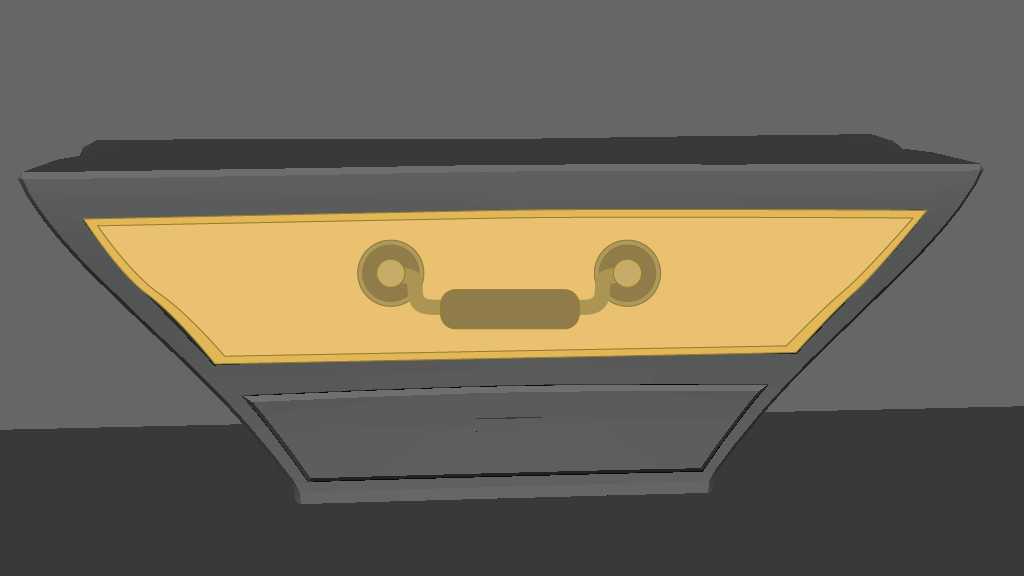
\includegraphics[width=.9\linewidth]{images/container_1}
    	\caption{Interactive but uncollectable drawer item}
    	\label{fig:uncollectable drawer}
    \end{subfigure}
	\begin{subfigure}{.45\textwidth}
		\centering
        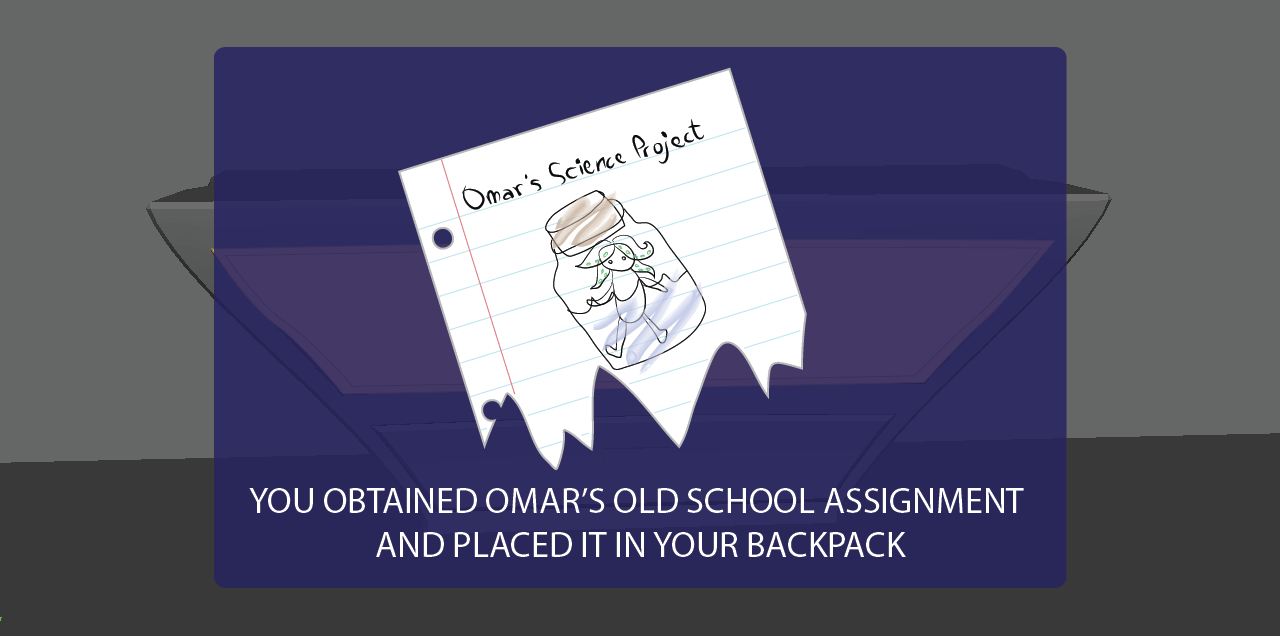
\includegraphics[width=.9\linewidth]{images/container_2}
    	\caption{Receiving an item from an uncollectable container item}
    	\label{fig:receive item}
    \end{subfigure}
    \caption{Example of an uncollectable item interaction}
    \label{fig:uncollectable}
\end{figure}